\clearpage

\section{Upsampler}

\begin{tcolorbox}	
	\begin{tabular}{p{2.75cm} p{0.2cm} p{10.5cm}} 	
		\textbf{Header File}   &:& upsampler.h \\
		\textbf{Source File}   &:& upsampler.cpp \\
        \textbf{Version}       &:& 20190319 (Daniel Pereira)\\
	\end{tabular}
\end{tcolorbox}

This block applies an interpolation filter.

\subsection*{Input Parameters}

\begin{table}[h]
\centering
\begin{tabular}{|c|c|p{60mm}|c|ccc}
\cline{1-4}
\textbf{Parameter} & \textbf{Type}   & \textbf{Values} & \textbf{Default} \\ \cline{1-4}
numberOfTaps       & int             & any             & 8                \\ \cline{1-4}
upSamplingFactor   & int             & any             & 2                \\ \cline{1-4}
\end{tabular}
\caption{Matched filter input parameters} 
\label{table:Upsampler}
\end{table}

\subsection*{Methods}

\bigbreak
Upsampler(initializer\_list$<$Signal *$>$ \&InputSig, initializer\_list$<$Signal *$>$ \&OutputSig) :Block(InputSig, OutputSig)\{\};
\bigbreak
void initialize(void);
\bigbreak
bool runBlock(void);
\bigbreak
void setNumberOfTaps(int numberOfTaps);
\bigbreak
void setUpsamplingFactor(int upSamplingFactor);

\subsection*{Functional description}


This block applies the FIR interpolation filter presented in Figure~\ref{fig:FILTER}.

\begin{figure}[h]
\centering
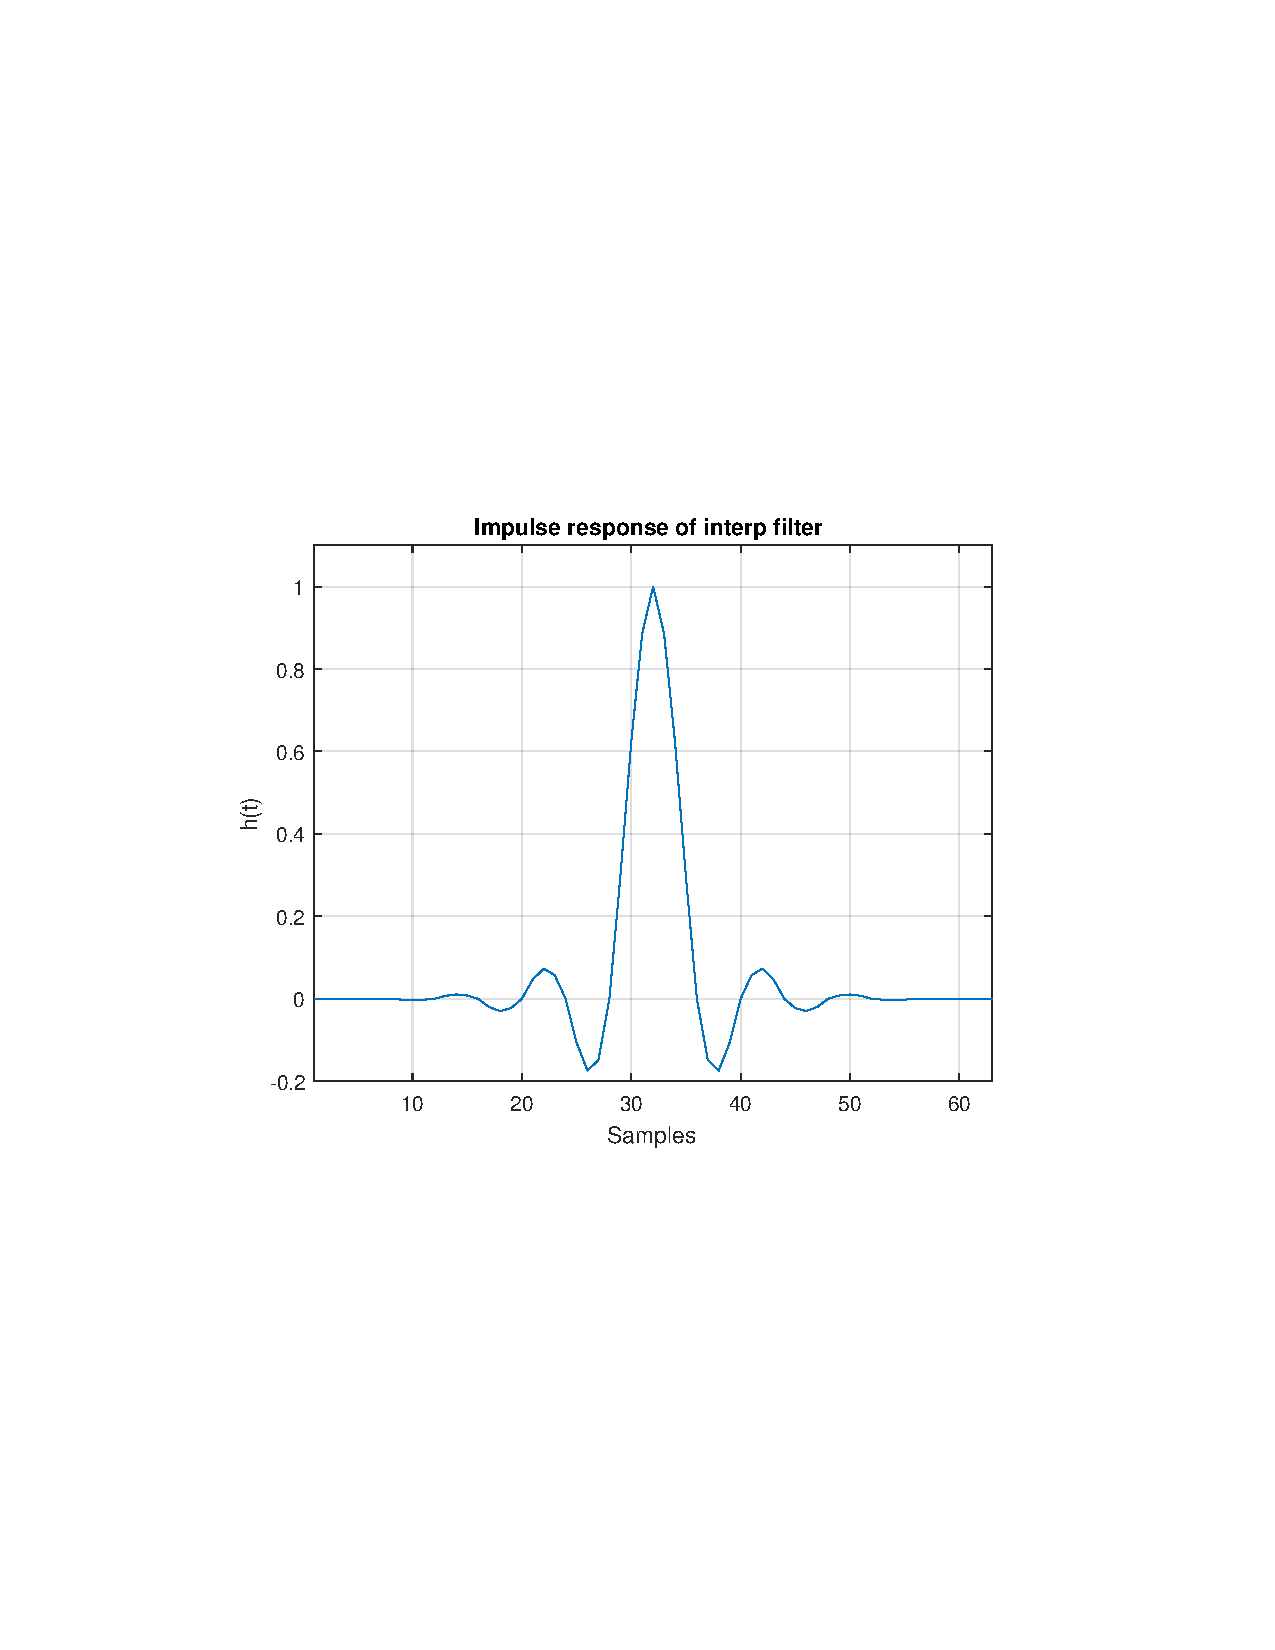
\includegraphics[trim={7cm 8cm 7cm 8cm},width=.3\linewidth]{./lib/upsampler/figures/FILTER}
\caption{Impulse response of a 4$\times$ upsampling filter using 16 taps.}
\label{fig:FILTER}
\end{figure}	

\subsection*{Input Signals}

\textbf{Number:} 1\\
\textbf{Type:} Complex signal

\subsection*{Output Signals}

\textbf{Number:} 1\\
\textbf{Type:} Complex signal

